\documentclass[10pt, conference, letterpaper]{IEEEtran}

\usepackage{algorithm}
\usepackage{algorithmicx}
\usepackage{algpseudocode}
\usepackage{amsfonts}
\usepackage{amsmath}
\usepackage{amssymb}
\usepackage[ansinew]{inputenc} 
\usepackage{xcolor}
\usepackage{mathtools}
\usepackage{graphicx}
\usepackage{caption}
\usepackage{subcaption}
\usepackage{import}
\usepackage{multirow}
\usepackage{cite}
\usepackage[export]{adjustbox}
\usepackage{breqn}
\usepackage{mathrsfs}
\usepackage{acronym}
%\usepackage[keeplastbox]{flushend}
\usepackage{setspace}
\usepackage{bm}
\usepackage{stackengine}

\usepackage{listings}

\lstset{%
 backgroundcolor=\color[gray]{.85},
 basicstyle=\small\ttfamily,
 breaklines = true,
 keywordstyle=\color{red!75},
 columns=fullflexible,
}%

\lstdefinelanguage{BibTeX}
  {keywords={%
      @article,@book,@collectedbook,@conference,@electronic,@ieeetranbstctl,%
      @inbook,@incollectedbook,@incollection,@injournal,@inproceedings,%
      @manual,@mastersthesis,@misc,@patent,@periodical,@phdthesis,@preamble,%
      @proceedings,@standard,@string,@techreport,@unpublished%
      },
   comment=[l][\itshape]{@comment},
   sensitive=false,
  }

\usepackage{listings}

% listings settings from classicthesis package by
% Andr\'{e} Miede
\lstset{language=[LaTeX]Tex,%C++,
    keywordstyle=\color{RoyalBlue},%\bfseries,
    basicstyle=\small\ttfamily,
    %identifierstyle=\color{NavyBlue},
    commentstyle=\color{Green}\ttfamily,
    stringstyle=\rmfamily,
    numbers=none,%left,%
    numberstyle=\scriptsize,%\tiny
    stepnumber=5,
    numbersep=8pt,
    showstringspaces=false,
    breaklines=true,
    frameround=ftff,
    frame=single
    %frame=L
}

\renewcommand{\thetable}{\arabic{table}}
\renewcommand{\thesubtable}{\alph{subtable}}

\DeclareMathOperator*{\argmin}{arg\,min}
\DeclareMathOperator*{\argmax}{arg\,max}

\def\delequal{\mathrel{\ensurestackMath{\stackon[1pt]{=}{\scriptscriptstyle\Delta}}}}

\graphicspath{{./figures/}}
\setlength{\belowcaptionskip}{0mm}
\setlength{\textfloatsep}{8pt}

\newcommand{\eq}[1]{Eq.~\eqref{#1}}
\newcommand{\fig}[1]{Fig.~\ref{#1}}
\newcommand{\tab}[1]{Tab.~\ref{#1}}
\newcommand{\secref}[1]{Section~\ref{#1}}

\newcommand\MR[1]{\textcolor{blue}{#1}}
\newcommand\red[1]{\textcolor{red}{#1}}
\newcommand{\mytexttilde}{{\raise.17ex\hbox{$\scriptstyle\mathtt{\sim}$}}}

%\renewcommand{\baselinestretch}{0.98}
% \renewcommand{\bottomfraction}{0.8}
% \setlength{\abovecaptionskip}{0pt}
\setlength{\columnsep}{0.2in}

% \IEEEoverridecommandlockouts\IEEEpubid{\makebox[\columnwidth]{PUT COPYRIGHT NOTICE HERE \hfill} \hspace{\columnsep}\makebox[\columnwidth]{ }} 

\title{``We Rock the Hizzle and Stuff'' \\ hints on how to write a nice research essay}

\author{Michele Rossi$^\dag$, Author two$^\ddag$
\thanks{$^\dag$Department of Information Engineering, University of Padova, email: \{rossi\}@dei.unipd.it}
\thanks{$^\ddag$Author two affiliation, email: \{name.surname\}@dei.unipd.it}
\thanks{Special thanks / acknowledgement go here.}
} 

\IEEEoverridecommandlockouts

\newcounter{remark}[section]
\newenvironment{remark}[1][]{\refstepcounter{remark}\par\medskip
   \textbf{Remark~\thesection.\theremark. #1} \rmfamily}{\medskip}

\begin{document}

\maketitle

\begin{abstract}
Future vehicular communication networks call for new solutions to support their capacity demands, by leveraging the potential of the \mbox{millimeter-wave} (\mbox{mm-wave}) spectrum. Mobility, in particular, poses severe challenges in their design, and as such shall be accounted for. A key question in \mbox{mm-wave} vehicular networks is how to optimize the \mbox{trade-off} between directive Data Transmission (DT) and directional Beam Training (BT), which enables it. In this paper, learning tools are investigated to optimize this \mbox{trade-off}. In the proposed scenario, a Base Station (BS) uses BT to establish a \mbox{mm-wave} directive link towards a Mobile User (MU) moving along a road. To control the BT/DT \mbox{trade-off}, a Partially Observable (PO) Markov Decision Process (MDP) is formulated, where the system state corresponds to the position of the MU within the road link. The goal is to maximize the number of bits delivered by the BS to the MU over the communication session, under a power constraint. The resulting optimal policies reveal that adaptive BT/DT procedures significantly outperform \mbox{common-sense} heuristic schemes, and that specific mobility features, such as user position estimates, can be effectively used to enhance the overall system performance and optimize the available system resources.\\ 

\MR{This is an example abstract. It is $204$ words long, I would say an abstract should not be longer than $250$ words and some Transactions journals of the IEEE are currently putting a strict limit of $200$ words. Here, you should briefly state: 
\begin{enumerate}
\item the technical scenario/field of research and its timeliness/relevance in general (one sentence),
\item what you do in the report/paper and why it is important, how it advances the state of the art in its field (a few sentences), 
\item summarize the main and best results of your study/proposal/method (one or two sentences),
\item (optional) how others could benefit from your results for further research, or within commercial products (one sentence).
\end{enumerate}  
The abstract is one of the most important parts of the paper/report. You have roughly one minute to catch the reader's attention. A poor abstract may already move you towards the rejection side in the reviewer's decision process. In the abstract, 1) establish the context, 2) motivate the problem, 3) briefly describe the solution, and 4) present the main results of your work. Ideally, use one (short) sentence for each of the previously mentioned items to keep your abstract short. Overall, this should be a short summary of the whole content of your paper, including your results.}\\

\MR{See the abstract as a personal challenge for each of your papers. Finally, the abstract should contain the main message about your work, so that the reader will now what she/he can find even without reading it (as it is the case most of the times). The abstract is a mini-paper on its own and, as such, it is a major endeavor to write.}\\ 

\red{I suggest to write the Abstract as the very last thing. You may sketch it at the beginning, but then always finalize it at the end.}
\end{abstract}

\IEEEkeywords
Self Organizing Maps, Unsupervised Learning, Optimization, Neural Networks, Recurrent Neural Networks. \MR{A list of keywords defining the tools and the scenario. I would not go beyond {\it six} keywords.}
\endIEEEkeywords


\input{Intro}

% !TEX root = template.tex

\section{Related Work}
Keyword spotting is used to detect specific words from a stream of  audio,  typically  in  a  low-power  always-on  setting  such  as smart speakers and mobile phones.   To achieve this,  audio is processed locally on the device.  In addition to detecting target words,  classifiers may also distinguish between ``silence'' and ``unknown'' for words or sounds that are not in the target list. In  recent  years,   machine  learning  techniques,   such  asdeep (DNN), convolutional (CNN) and recurrent (RNN) neu-ral  networks,  have  proven  to  be  useful  for  keyword  spotting. These networks are typically used in conjunction with a pre-processing pipeline which extracts the mel-frequency cepstrumcoefficients (MFCC) \cite{davis1980comparison}. 


Deep learning models have shown state-of-the-art performance in KWS \cite{hinton2012deep}, \cite{sainath2013deep}. 



The authors in \cite{chen2014small} have proposed a low-latency keyword detection method for mobile users using a deep learning-based technique and termed it as ‘deep KWS’. The deep KWS method has not only been proven suitable for low-powered embedded systems but also has outperformed the baseline Hidden Markov Models for both noisy and noise-free audio data. The deep KWS uses a fully connected DNN with transfer learning  based on speech recognition. The network is further optimized for KWS with end-to-end fine-tuning using stochastic gradient descent. Sainath et al. \cite{sainath2015convolutional} have introduced a similarly small footprint KWS system based on CNNs. Their proposed CNN uses fewer parameters than a standard DNN model, which makes the proposed system more attractive for platforms with resource constraints. 
The DNN is a standard feed-forward neural network made of a stack of fully-connected layers andnon-linear activation layers. The input to the DNN is the flattened feature matrix, which feeds into astack ofdhidden fully-connected layers each withnneurons. Typically, each fully-connected layeris followed by a rectified linear unit (ReLU) based activation function. At the output is a linear layerfollowed by a softmax layer generating the output probabilities of thekkeywords, which are used forfurther posterior handling.3.2  Convolutional Neural Network (CNN)One main drawback of DNN based KWS is that they fail to efficiently model the local temporaland spectral correlation in the speech features. CNNs exploit this correlation by treating the inputtime-domain and spectral-domain features as an image and performing 2-D convolution operationsover it.  The convolution layers are typically followed by batch normalization [17], ReLU basedactivation functions and optional max/average pooling layers, which reduce the dimensionality ofthe features. During inference, the parameters of batch normalization can be folded into the weightsof the convolution layers. In some cases, a linear low-rank layer, which is simply a fully-connectedlayer without non-linear activation, is added in between the convolution layers and dense layers forthe purpose of reducing parameters and accelerating training  [18, 19].3.3  Recurrent Neural Network (RNN)RNNs have shown superior performance in many sequence modeling tasks, especially speech recogni-tion [20], language modeling  [21], translation [22], etc. RNNs not only exploit the temporal relationbetween the input signal, but also capture the long-term dependencies using "gating" mechanism.Unlike CNNs where input features are treated as 2-D image, RNNs operate forTtime steps, whereat each time steptthe corresponding spectral feature vectorft∈RFconcatenated with the previoustime step outputht−1is used as input to the RNN. Figure 2 shows the model architecture of a typicalRNN model, where the RNN cell could be an LSTM cell [23,24] or a gated recurrent unit (GRU)cell [25,26]. Since the weights are reused across all theTtime steps, the RNN models tend to haveless number of parameters compared to the CNNs. Similar to batch normalization in CNNs, researchshow that applying layer normalization can be beneficial for training RNNs [27], in which the hiddenstates are normalized during each time step


% !TEX root = template.tex

\section{Processing Pipeline}
\label{sec:processing_architecture}
 Conceptually, our system consistsof three components.   First,  in the feature extraction module,40 dimensional log-mel filterbank features are computed every25ms with a 10ms frame shift.  Next, at every frame, we stack23 frames to the left and 8 frames to the right, and input thisinto the DNN
 
 
CNN is an image classification technique and one of the major challenges in speech and acoustic event recognition has been how to best represent the audio signal using an image for this purpose. Two common approaches have been seen in addressing this problem. Firstly, the audio signal is converted to spectrogram images \cite{zhang2015robust}. Secondly, a mel-filter, as used in computing mel-frequency cepstral coefficients (MFCC), is used to form an image-like representation \cite{abdel2014convolutional]}.  To ensure that all images are of an equal size, the audio signal is divided into a fixed number of frames \cite{We refer this as the mel-spectrogram.}.


CNNs run a small window over the input image atboth training and testing time, so that the weights of the networkthat looks through this window canlearn from various featuresof the input data regardless of their absolute position within theinput.Weight sharing, or to be more precise in our present situ-ation,full weight sharingrefers to the decision to use the sameweights at every positioning of the window. CNNs are also often said to be local because the individual units that are computed at a particular positioning ofthe window depend upon featuresof the local region of the image that the window currently looksupon.
 Time presents no immediate problem from the standpoint of locality. Likeother DNNs for speech, a single window of input to the CNNwill consist of a wide amount of context (9–15 frames). Asfor frequency, the conventional use of MFCCs does present amajor problem because the discrete cosine transform projectsthe spectral energies into a new basis that may not maintain lo-cality. In this paper, we shall use the log-energy computed di-rectly from the mel-frequency spectral coefficients (i.e., with noDCT), which we will denote asMFSC features. These will beused to represent each speech frame in order to describethe acoustic energy distributionin each of several different frequency bands

There exist several different alternatives to organizing theseMFSC features into maps for the CNN. First, as shown inFig. 1(b), they can be arranged as three 2-D feature maps,each of which represents MFSC features (static, delta anddelta-delta) distributed along both frequency (using the fre-quency band index) and time (using the frame number withineach context window). In this case, a two-dimensional con-volution is performed (explained below) to normalize bothfrequency and temporal variations simultaneously. 


We evaluated our models using Google’s Speech CommandsDataset  [9],  which  was  released  in  August  2017  under  aCreative  Commons  license.2The  dataset  contains  65,000one-second long utterances of 30 short words by thousands ofdifferent people, as well as background noise samples such aspink noise, white noise, and human-made sounds.  The blogpost  announcing  the  data  release  also  references  Google’sTensorFlow implementation of Sainath and Parada’s models,which provide the basis of our comparisons


The output of each must be post-processed

\section{Signals and Features}
For  feature  extraction,   we  first  apply  a  band-pass  filterof  20Hz/4kHz  to  the  input  audio  to  reduce  noise.    Forty-dimensional  Mel-Frequency  Cepstrum  Coefficient  (MFCC)frames are then constructed and stacked using a 30ms win-dow and a 10ms frame shift.  All frames are stacked across a1s interval to form the two-dimensional input to our models.
For the speech regions, we generate acoustic features based on40-dimensional log-filterbank energies computed every 10 ms overa window of 25 ms. Contiguous frames are stacked to add sufficientleft and right context. The input window is asymmetric since eachadditional frame of future context adds 10 ms of latency to the sys-tem. For our Deep KWS system, we use 10 future frames and 30frames in the past.
A  block  diagram  of  the  DNN  KWS  system  [2]  used  in  thiswork is shown in Figure 1. 




In this work, we focus on convolutional neural networks(CNNs), a class of models that has been successfully appliedto small-footprint keyword spotting in recent years.  In par-ticular, we explore the use of residual learning techniques anddilated convolutions. On the recently-released Google SpeechCommands  Dataset,  which  provides  a  common  benchmarkfor keyword spotting, our full residual network model outper-forms Google’s previously-best CNN [1] (95.8% vs. 91.7% inaccuracy).  We can tune the depth and width of our networksto target a desired tradeoff between model footprint and ac-curacy: one variant is able to achieve accuracy only slightlybelow Google’s best CNN with a 50×reduction in model pa-rameters and an 18×reduction in the number of multipliesin a feedforward inference pass.  This model far outperformsprevious compact CNN variants


\section{Learning Framework}
The model presented in \cite{sainath2015convolutional} is a CNN architecture that address the constraints of each applications. We find that theCNN architectures offer between a 27-44% relative improve-ment in false reject rate compared to a DNN, while fitting intothe constraints of each application

\subsection{Residual layers}
\subsection{Attention layers}
\subsection{Inception-like layers}


% !TEX root = template.tex

\section{Results}
\label{sec:results}

%In this section, you should provide the numerical results. You are free to decide the structure of this section. As a general ``rule of thumb'', use plots to describe your results, showing, e.g., precision, recall and \mbox{F-measure} as a function of the system (learning) parameters. You can also show the precision matrix. 


The results obtained with these models are shown in Table \ref{table:results}, which also shows the 95\% confidence intervals from tree  different trials.

\begin{table}
	\centering
	\begin{tabular}{|l|l|l|l|}
    \hline
    model  & parameters & accuracy  & time \\
    \hline
    res3 & 20,380 & 0.8445 & 5849ms \\
    \hline
    res6 & $3^1$ & $3c\dfrac{n}{3}$ & $3^0$\\
    \hline
    res9 & $3^2$ & $9c\dfrac{n}{3^2}$ & $3^0$ \\
    \hline
    vit5x4 & $3^i$ & $3^ic\dfrac{n}{3^i}=cn$ & $3^0$  \\
    \hline
    vit10x8  & $3^i$ & $3^ic\dfrac{n}{3^i}=cn$ & $3^0$  \\
    \hline
    vit20x10  & $3^i$ & $3^ic\dfrac{n}{3^i}=cn$ & $3^0$  \\
    \hline
    \end{tabular} 
\label{table:results}
\caption{Results obtained per each model over 3 trials}
\end{table}


\begin{figure}[h]
    \centering
    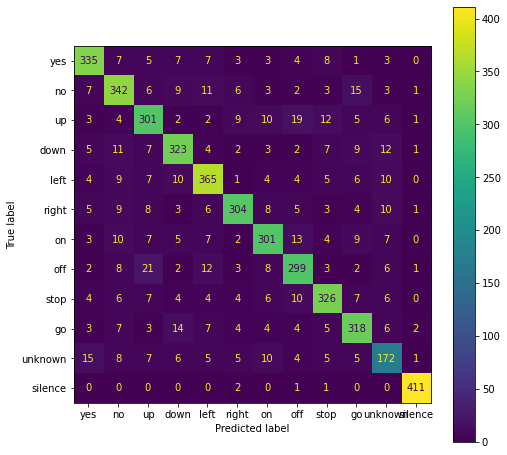
\includegraphics[width=0.5\textwidth]{confusion_matrix_res3_keyword.png}
    \label{fig:confusionmatrix}
    \caption{Confusion Matrix of the model res3}
\end{figure}


Checking the confusion matrix of model res3 \ref{fig:confusionmatrix}, we can observe well the accuracy is no so high. We can notice that the best label that the model predicts is unknown, and also we can observe that the model sometimes doesn't predict well for labels off and up.  

%
%\begin{remark}
%Present the material in a progressive and logical manner, starting with simple things and adding details and explaining more complex findings as you go. Also, do not try to explain/show multiple concepts within the same sentence. Try to \textbf{address one concept at a time}, explain it properly, and only then move on to the next one.
%\end{remark}
%
%\begin{remark}
%The best results are obtained by generating the graphs using a vector type file, commonly, either \texttt{encapsulated postscript (eps)} or \texttt{pdf} formats. To plot your figures, use the Latex \texttt{\textbackslash includegraphics} command. Lately, I tend to use pdf more.
%\end{remark}
%
%\begin{remark}
%If your model has hyper-parameters, show selected results for several values of these. Usually, tables are a good approach to concisely visualize the performance as hyper-parameters change. It is also good to show the results for different flavors of the learning architecture, i.e., how architectural choices affect the overall performance. An example is the use of CNN only or CNN+RNN, or using inception for CNNs, dropout for better generalization or attention models. So you may obtain different models that solve the same problem, e.g., CNN, CNN+RNN, CNN+inception, etc.
%\end{remark}


% !TEX root = template.tex

\section{Concluding Remarks}
\label{sec:conclusions}

\red{This section should take max half a page, I personally find it difficult to come up with really useful observations, I mean ones that bring a new contribution with respect to what you have already expounded in the ``Results'' section. In case you have some serious stuff to write, you may also extend the section to 3/4 of a page :-).}\\

In many papers, here you find a summary of what done. It is basically an abstract where instead of using the present tense you use the past participle, as you refer to something that you have already developed in the previous sections. While I did it myself in the past, I now find it rather useless.\\ 

\MR{\textbf{What I would like to see here is:} 
\begin{enumerate}
\item a very short summary of what done, 
\item some (possibly) intelligent observations on the relevance and {\it applicability} of your algorithms / findings, 
\item what is still missing, and can be added in the future to extend your work.\\
\end{enumerate}
The idea is that this section should be {\it useful} and not just a repetition of the abstract (just \mbox{re-phrased} and written using a different tense...).}\\

\red{\textbf{Moreover:} being a project report, I would also like to see a specific paragraph stating 
\begin{enumerate}
\item[4)] what you have learned, and 
\item[5)] any difficulties you may have encountered.
\end{enumerate}}


\section{Exam rules}

What you need to do to pass the exam:
\begin{itemize}
\item Optional: team up with another student. Max. group size is \textbf{two students} per group;
\item Identify a project to work on, devise your own neural network architecture and test it on the provided dataset;
\item \textbf{Prepare a written project report} including: i) diagrams, ii) configuration pars, iii) results, iv) your discussion;
\item \textbf{Prior to presenting your work}: upload i) your written report and ii) the code;
\item \textbf{Present your work} using slides (max. duration is 20 minutes): take turns in presenting your work, your individual contribution to the project should clearly emerge. Optional: a final and quick demo with running code is appreciated and will be considered in the calculation of the final grade (see below). 
\end{itemize}

Your final grade will be obtained taking into account the following criteria:
\begin{itemize} 
\item \textbf{Project} (60 points): originality (10 pt.) - data preprocessing techniques (10 pt.) - learning architectures (20 pt.) - comparison against other/existing approaches (10 pt.) - live demo of the code (10 pt.)
\item \textbf{Written report} (40 points): clarity of exposition (10 pt.) - completeness (10 pt.) - analysis of results (number and type of metrics used) (20 pt.)
\item \textbf{Oral exposition} (20 points): duration (your talk must take max. 20 minutes, using slides) (10 pt.) - clarity of exposition (10 pt.)
\end{itemize}

The final grade will be computed as
\begin{equation}
\textrm{grade} = \frac{\textrm{tot\_points} \times 30}{110}
\end{equation}

\bibliography{biblio}
\bibliographystyle{ieeetr}

\end{document}


